\documentclass[crop, tikz, convert=pdf2svg]{standalone}
\usetikzlibrary{calc,positioning,fit,backgrounds,shapes.symbols}
\begin{document}
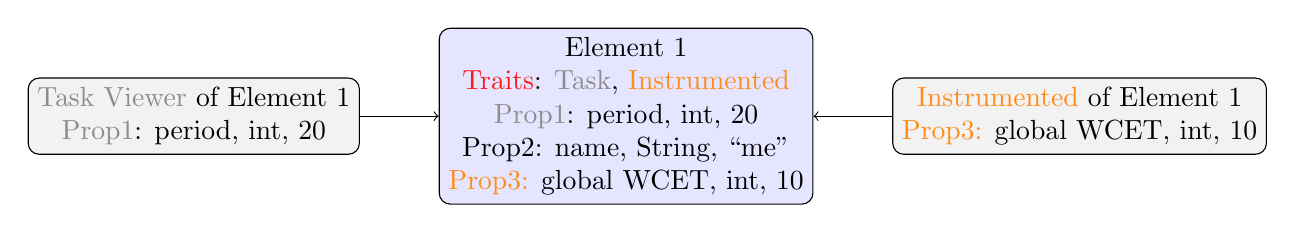
\begin{tikzpicture}[
elem/.style={rounded corners, fill=blue!10, draw=black, align={center}},
viewer/.style={rounded corners, fill=gray!10, draw=black, align={center}}
]
\node[elem] (element) {
    Element 1\\
    {\color{red!90} Traits}: {\color{gray!90} Task}, {\color{orange!90} Instrumented}\\
    {\color{gray!90} Prop1}: period, int, 20\\
    Prop2: name, String, ``me''\\
    {\color{orange!90} Prop3:} global WCET, int, 10
};
\node[viewer, left=1 of element] (taskviewer) {
    {\color{gray!90} Task Viewer} of Element 1\\
    {\color{gray!90} Prop1}: period, int, 20
};
\node[viewer, right=1 of element] (instruviewer) {
    {\color{orange!90} Instrumented} of Element 1\\
    {\color{orange!90} Prop3:} global WCET, int, 10
};
\draw[->] (taskviewer) -- (element);
\draw[->] (instruviewer) -- (element);
\end{tikzpicture}
\end{document}